
\documentclass[11pt]{article}


\usepackage[utf8x]{inputenc}
\usepackage{hyperref}
\usepackage{amsmath}
\usepackage{amssymb} 
\usepackage{textcomp}
\usepackage[francais]{babel}
\usepackage{natbib} 
\usepackage{hyperref} 


\usepackage{graphicx}
\graphicspath{ {./} }
\usepackage{wrapfig}
\usepackage[top=0.8in, bottom=0.8in, left=0.8in, right=0.8in]{geometry}


\title{La Suisse comme paradis fiscal au XXe siècle dans le
\textit{Journal de Genève} et la \textit{Gazette de Lausanne}}
\author{Yann Bolliger, Pietro Carta, Romain Mendez}

\begin{document}
\maketitle

\section{Contexte historique}

La place financière suisse a vu une énorme croissance presque non perturbée tout
au long du XXème siècle. Cela a été possible grâce à la neutralité et la
stabilité de la Suisse notamment en période de guerre mais surtout aussi grâce
au «secret bancaire»~\citep[p. 512]{Mazbouri12}. Ce dernier
est déjà une pratique des banques suisses au XIXème siècle quand les grandes
banques\footnote{Union de Banques Suisses, Schweizerische Kreditanstalt (Crédit
Suisse), Schweizerische Volksbank, Banque Leu, Eidgenössische Bank, Société de
Banque Suisse, Banque Commerciale de Bâle et le Comptoir d’Escompte} commencent
à dominer la place financière suisse. Ces banques-là profitent considérablement
des afflux de capitaux étrangers. Pendant la Grande Guerre ou les banques utilisent
le secret bancaire pour attirer les capitaux étrangers fuyant de lourdes
fiscalités implémentées par les pays en guerre~\citep[p. 484-486]{Mazbouri12}.

Cela leur permet de devenir une force majeur à l’échelle de la finance mondiale
ainsi qu’une qu’une influence principale dans la politique nationale. En effet,
l’influence des banques dans la politique fédérale est tellement grande que
le secret bancaire est renforcé par la loi sur les banques en 1934, sans
susciter de grands débats au parlement~\citep{Guex99}. 

Avec la seconde guerre mondiale, de nouveau, la place financière Suisse profite
à nouveau de la fuite de capitaux étrangers provenant de pays en guerre. Sous
couvert de la neutralité, les banques suisses arrivent à maintenir des liens
très proches avec tous les belligérants, mais surtout avec les forces de l’Axe.
Ce qui mène la suisse dans une grande isolation diplomatique à la fin de la
guerre. Par exemple, les États-unis gèlent les avoirs des banques suisses
déposés en Amérique déjà en 1941. Néanmoins la diplomatie Suisse obtient le
maintien du secret bancaire contre les revendications des vainqueurs. Cela
marque le début d’une période de croissance sans précédent pour la place
financière pendant les «trente glorieuses»~\citep[p. 495]{Mazbouri12}.

Mais après la guerre, à l'étranger, le secret bancaire suisse reste objet de
fortes critiques. Les plus importants critiques étant les États-unis et la
France~\citep[p.503]{Mazbouri12}. Dans la deuxième partie du XXe siècle, la
diplomatie américaine obtient de la Suisse quelques concessions qui ont
toutefois très peu d'impact.  Après 1968, des critiques intérieures commencent
a troubler le consensus de la population suisse à faveur du secret bancaire.
L’organisation tiers-mondiste “Déclaration de Berne”\footnote{une bref histoire
de l'organisation est disponible sur DHS \citep{EvB}} se bats contre
l'exploitation des pays en voi de développement par le secteur financier et
industrial suisse. Cette organisation lance, conjointement avec le Parti
Socialiste, une initiative populaire contre le secret bancaire en
1984\footnote{Initiative populaire ``contre l'abus du secret bancaire et de la
puissance des banques''.
https://www.bk.admin.ch/ch/f/pore/va/19840520/index.html}. L'initiative
populaire est toutefois rejeté par une forte majorité des suisse (70\%).


Les grandes banques et les élites politiques ont ainsi réussi à maintenir ce
statut privilégié de la place financière pendant plus que 50 ans. Ils l’ont
défendu contre la pression de l’intérieur et de l’extérieur et ce n’est
seulement après la crise financière en 2007 que le secret est levé.

Dans le cadre de notre recherche nous essayerons de retrouver ces événements
dans la presse romande. Celle-ci étant plutôt proche des cercles financiers –
surtout le «journal de Genève» \citep{ConfClass1} –, nous évaluerons aussi
leurs positions sur le secret bancaire et si cette proximité peut-être
confirmée par les articles du corpus. Afin de nous demander, comment évolue la
couverture médiatique du secret bancaire au XXe siècle ? 

\section{Information Bibliographiques et de Corpus}
Nous admettons dans notre analyse les articles extrait de la “Gazette de
Lausanne” et du “Journal de Genève”, issus dans les deux journaux pendants la
période 1900-1995. Pour restreindre l’analyse aux article pertinents, le corpus
d’articles des deux journaux sera filtré en ne gardant que les articles
contenant des mots clés, repérés à travers l’analyse de nos autres sources
primaires et secondaires.

Les sources primaire que nous analysons, outres que les archives du Temps, sont
de nature politique, juridiques, ou diplomatique.

La “Déclaration de Berne” en collaboration avec le
Parti Socialiste publie en 1978 le pamphlet “Les Secrets du secrets bancaire
suisse” \citep{GiovanniniPierLuigi1978Lsds} où les conséquences internationales
et intérieures du secret bancaire sont dénoncé. Cet ouvrage nous expose au
discour qui entourait le sujet pendants les années 70s et 80s. Un nombre de
scandale pertinents au secret bancaire en sont les protagonistes.

Les sources juridiques nous témoignent d'un conflit entre la Suisse et des pays
étranger dans le domaine du secret bancaire. La sentence du tribunal fédéral. 
La sentence du tribunal fédéral \citep{tribunalFederal70} en faveur du maintien 
du secret bancaire en 1970 nous montre que la loi est appliqué avec conviction.

Nous étudierons aussi l'accord bilatéral entre la Suisse et les Etats-Unis sur
le secret bancaire, comme témoigné dans un rapport du \citet{insiderTrading83}.

L’histoire financière suisse a été étudié extensivement par Sébastien Guex et
Malik Mazbouri \citep{Guex99} \citep{Guex00} \citep{Mazbouri12}.
Les aspects juridiques du secret bancaire ont été déja étudié en 1969
par \citet{Mueller69}.
La spécificité du cas suisse au niveau international est analysé par
Meier \citep{Meier12}.

Mots clés: secret bancaire, place financière suisse, banques suisses, forfait
fiscal, liechtenstein, impôt anticipé, pots-de-vin, manipulation boursières,
paradis fiscal, compensateurs, corruption, affaire chiasso, argent sale,
blanchiment.

\section{Outils Méthodologiques}

Afin de pouvoir traiter en un temps raisonnable notre corpus de texte, plusieurs
pistes d’analyse s’offrent à nous. Dans un premier temps un filtrage des
articles s’impose, pour ne travailler que sur des articles contenant des termes
importants du sujet (voir la liste de terme clés dans la précédente partie).

Ensuite, nous pensons procéder à des visualisations du corpus filtré avec des
logiciels tel que Iramuteq afin de voir les relations entre les mots (quels mots
se suivent souvent, et quelle est leur connotation).

Avec de telles visualisation nous voulons aussi que cela nous permette de
trouver plus de mots-clés, par exemple dans la Figure 1. Nous pouvons voir que
les mots Secret et Bancaire sont peu liée au mots initiative populaire en 1984
(alors que c'est une année d'initiative populaire sur le sujet du secret
bancaire). Ici on peut voir que les thèmes en question sont toujours liés à la
Suisse en elle-même. Dans les mots autour de "initiative" on peut trouver
d'autres mots forts comme "balayer" ou "socialiste", ce qui indique par exemple
une certaine position dans les articles parlant de l'initiative.

Nous voulons tenter de répondre aux questions suivantes : A qui est-ce que la
parole est-elle donnée dans les journaux ? Est-ce que les acteurs étrangers
s'expriment ? Et surtout est-ce que les banques sont promues ?

Cette dernière question nous amène à nous demander, comment détecter si les
banques sont promues et/ou critiquée ? L'idée actuelle est de voir si des
mots-clés traditionnellement associé au point de vu positif sont dans les
articles abordant le sujet ou non (tel que PIB, emploi, croissance ...).
    
Nous pensons donc utiliser les sources secondaires pour forger une attente du
corpus, ceux à quoi nous nous attendons après ce type d’analyse. C’est à dire
par exemple utiliser les informations recueillies sur les rédactions des
journaux dans la conférence du 31 Octobre “Un parcours singulier dans l'histoire
de la presse romande: "Gazette de Lausanne" (1798-1991) et "Journal de Genève
(1826-1998)” par Prof. Alain Clavien afin de vérifier nos résultats avec les
différentes tendances des rédactions de ces deux journaux. Cela devrait pouvoir
nous servir de garde-fou sur nos résultats. Une fois ce travail accompli, nous
nous servirons des résultats pour analyser la position idéologique des journaux
au fil du temps dans la période étudiée. 

\begin{figure}
  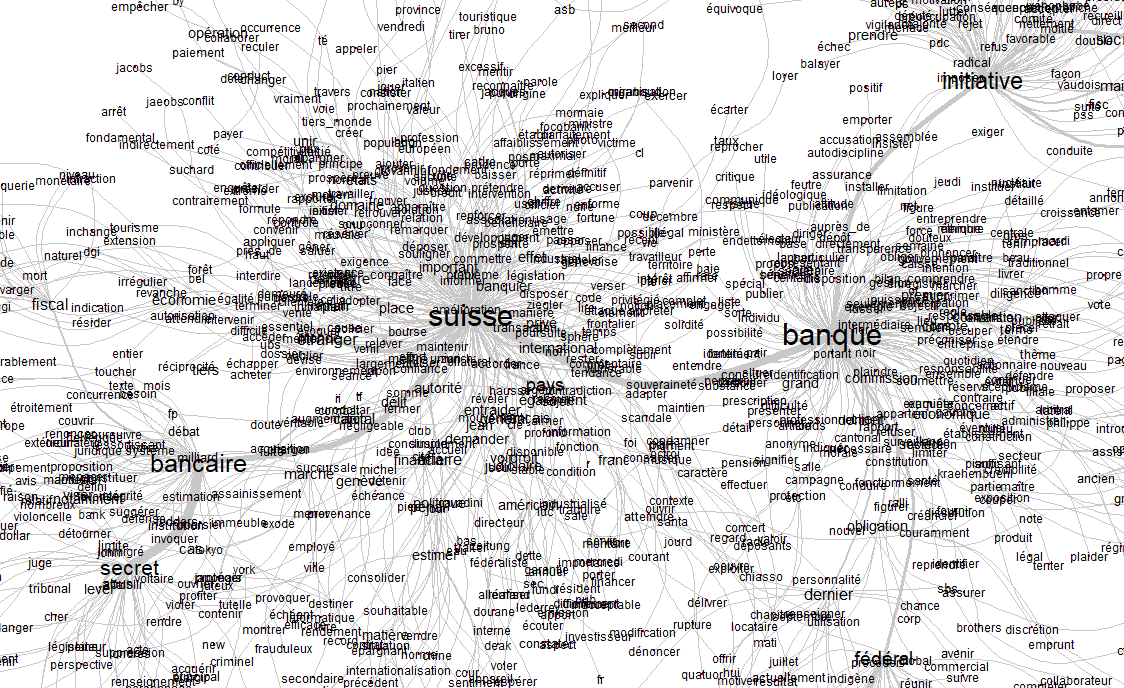
\includegraphics[width=7in]{reduced.png}
  \caption{Zoom dans la visualisation sur les articles contenant les mots "secret 
bancaire" dans l'année 1984 dans le \textit{Journal de Genève}}
\end{figure}

\bibliographystyle{agsm}
\bibliography{bib/bibliography}

\end{document}
